\section{Pianificazione}
La pianificazione del progetto viene suddivisa nelle seguenti fasi:
\begin{itemize}
	\item \textbf{Analisi;}
	\item \textbf{Presentazione;}
	\item \textbf{Progettazione architetturale;}
	\item \textbf{Progettazione di dettaglio e codifica;}
	\item \textbf{Validazione e collaudo.}
\end{itemize}
Ogni fase ha la sua corrispettiva scadenza (vedi 1.5) e viene suddivisa in sotto-attività prima di iniziare la sua implementazione.
\subsection{Analisi}
\begin{figure}[h!]
	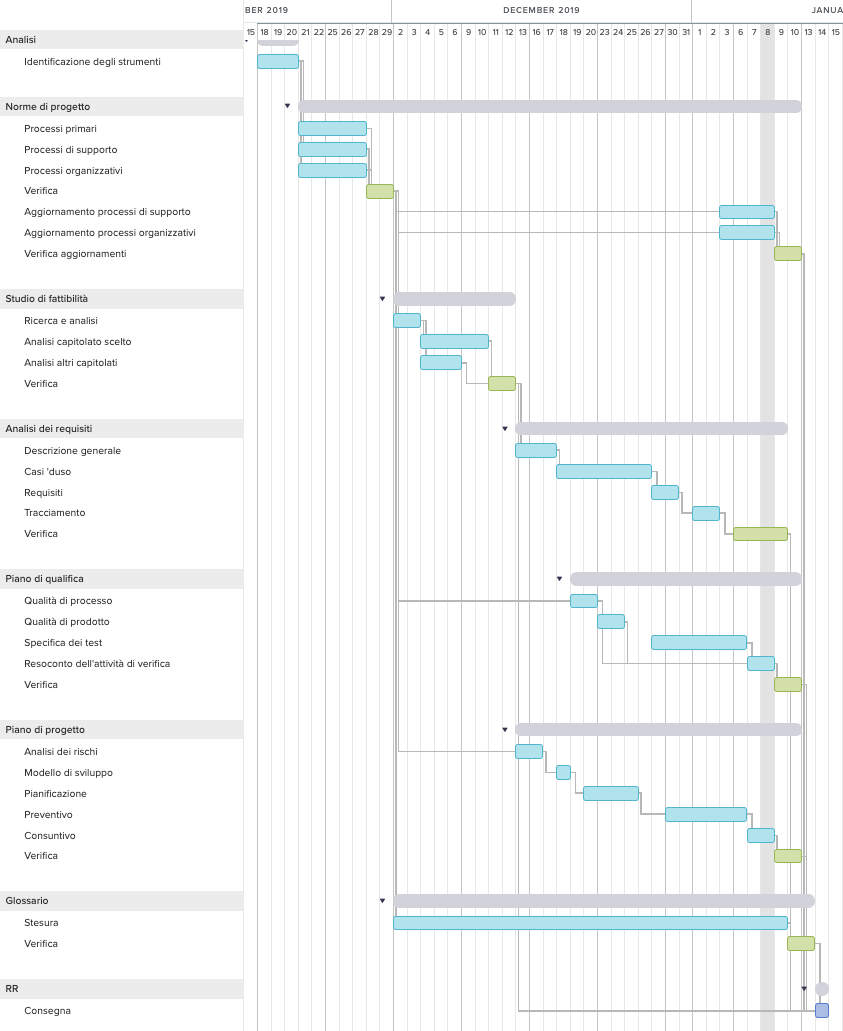
\includegraphics[width=\textwidth]{res/img/g1113}
	\caption{Pianificazione fase di Analisi}
\end{figure}
Questa fase è stata suddivisa nelle attività:
\begin{itemize}
	\item \textbf{Individuazione degli strumenti:} questa attività consiste nel determinare quali strumenti il gruppo deve utilizzare per la comunicazione, per la stesura dei documenti, per il versionamento, lo sviluppo e la verifica del software;
	\item \textbf{Norme di Progetto:} sono definite tutte le regole utili per lo svolgimento del progetto, relative al prodotto da realizzare e ai processi da adottare. Il documento \textit{Norme di Progetto X.X.X}\doc viene redatto dall'Amministratore per conto del Responsabile di progetto e viene costantemente aggiornato;
	\item \textbf{Studio di fattibilità:} in questa attività gli analisti effettuano uno studio approfondito dei capitolati in modo da determinare quale di essi verrà scelto. Questa attività è da considerarsi bloccante per l’attività di Analisi dei Requisiti;
	\item \textbf{Analisi dei Requisiti:} durante questa attività vengono identificati ed analizzati i requisiti del capitolato scelto nell'attività di studio di fattibilità e il relativo documento viene composto dagli Analisti;
	\item \textbf{Piano di Qualifica:} in questa attività si individuano le metodologie attraverso le quali si garantisce la qualità del prodotto. A supporto di ciò viene redatto il documento Piano di Qualifica da parte dell'Amministratore e per la parte programmatica dal Progettista;
	\item \textbf{Glossario:} tutti i termini che possono risultare ambigui vengono individuati e definiti nel documento \textit{Glossario 1.0.0}\docs, che viene redatto durante tutta la fase di analisi dei requisiti.
\end{itemize}

\newpage
\subsection{Presentazione RR}
\begin{figure}[h!]
	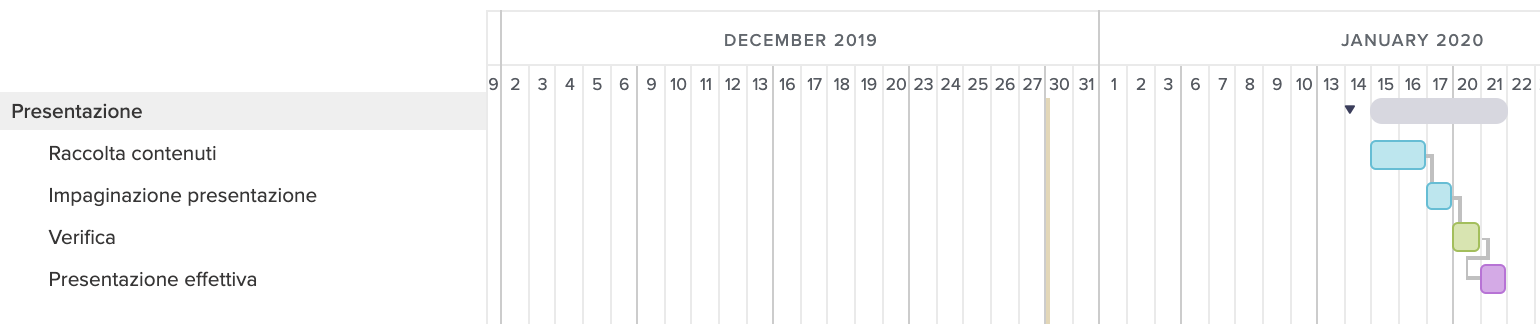
\includegraphics[width=\textwidth]{res/img/g2}
	\caption{Pianificazione presentazione RR}
\end{figure}
Viene fornita una pianificazione per la predisposizione e preparazione dei contenuti per la presentazione alla revisione formale.

\subsection{Progettazione architetturale}
\begin{figure}[h!]
	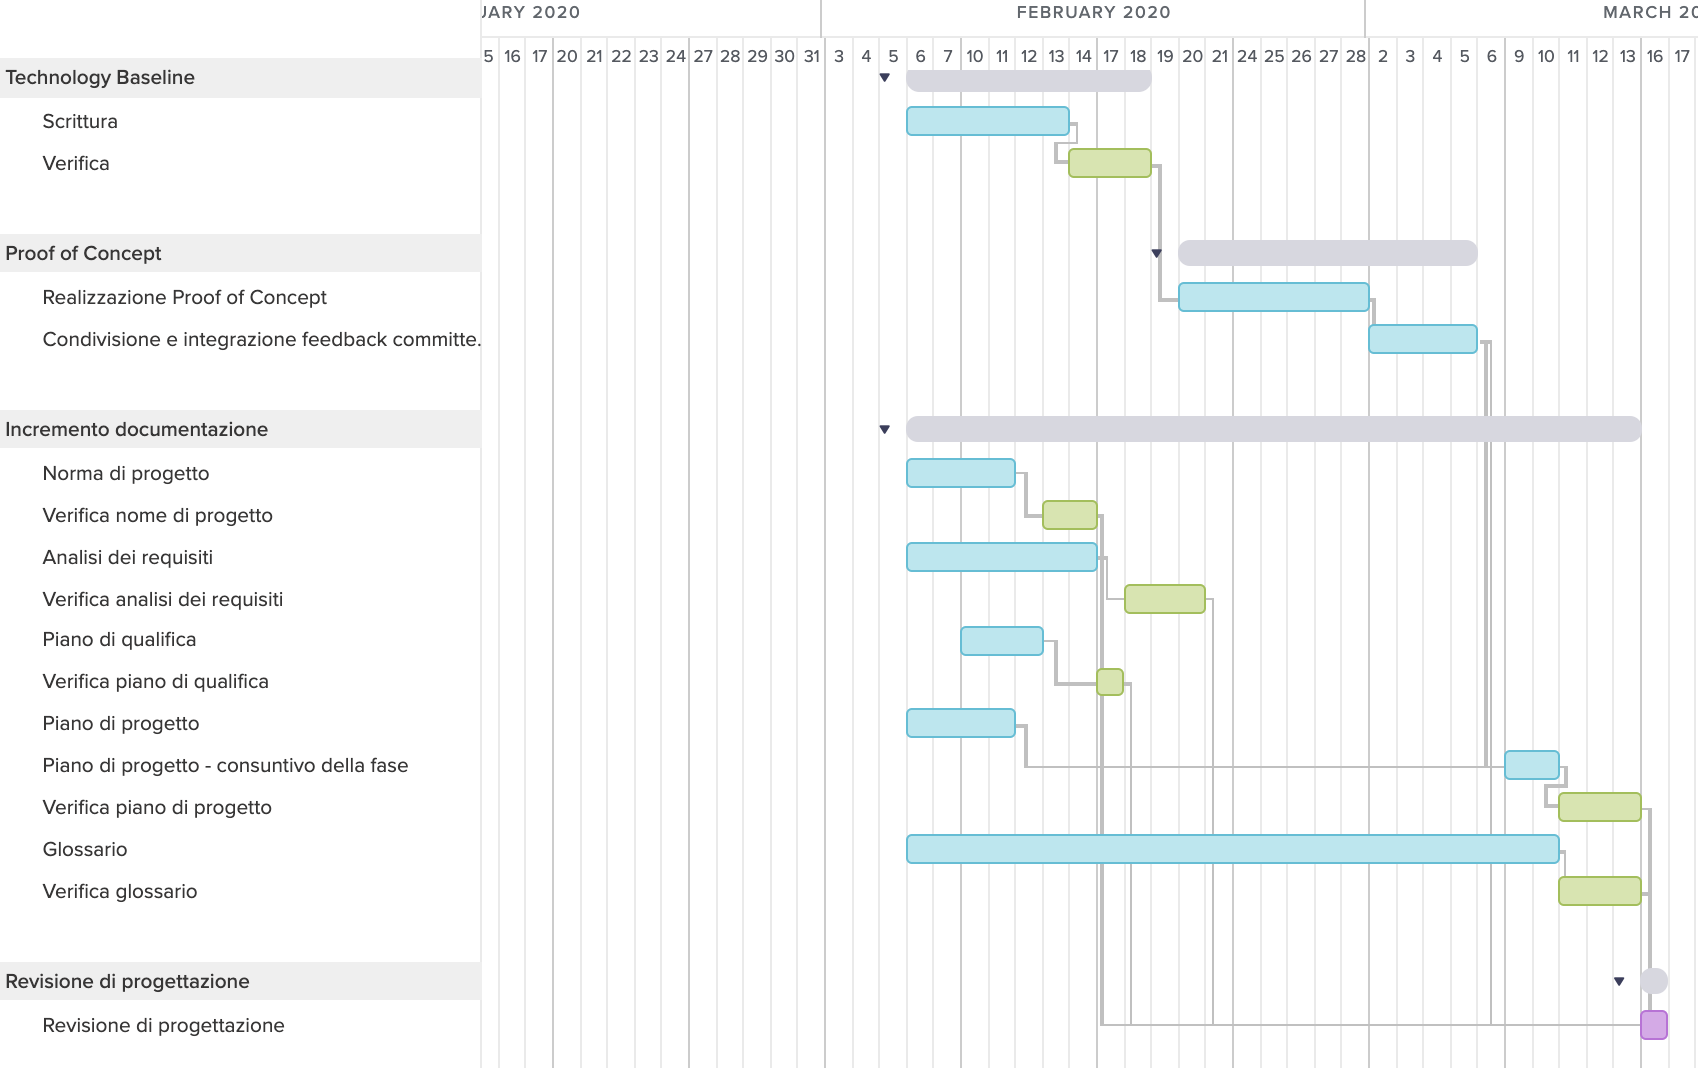
\includegraphics[width=\textwidth]{res/img/g3}
	\caption{Pianificazione Progettazione architetturale}
\end{figure}
Questa fase consiste nell'individualizzazione di una soluzione architetturale che soddisfi i requisiti del prodotto ed è stata suddivisa nelle sotto-attività:
\begin{itemize}
	\item \textbf{Technology Baseline:} redazione di un documento nel quale vengono individuati e specificati i pattern architetturali utilizzati negli ambiti delle tecnologie coinvolte;
	\item  \textbf{Proof of concept:} codifica di una bozza del prodotto per verificare la correttezza dell'architettura del sistema;
	\item \textbf{Documentazione:} incremento della documentazione in base ai nuovi dati rilevati.
\end{itemize}


\subsection{Progettazione di dettaglio e codifica}
\begin{figure}[h!]
	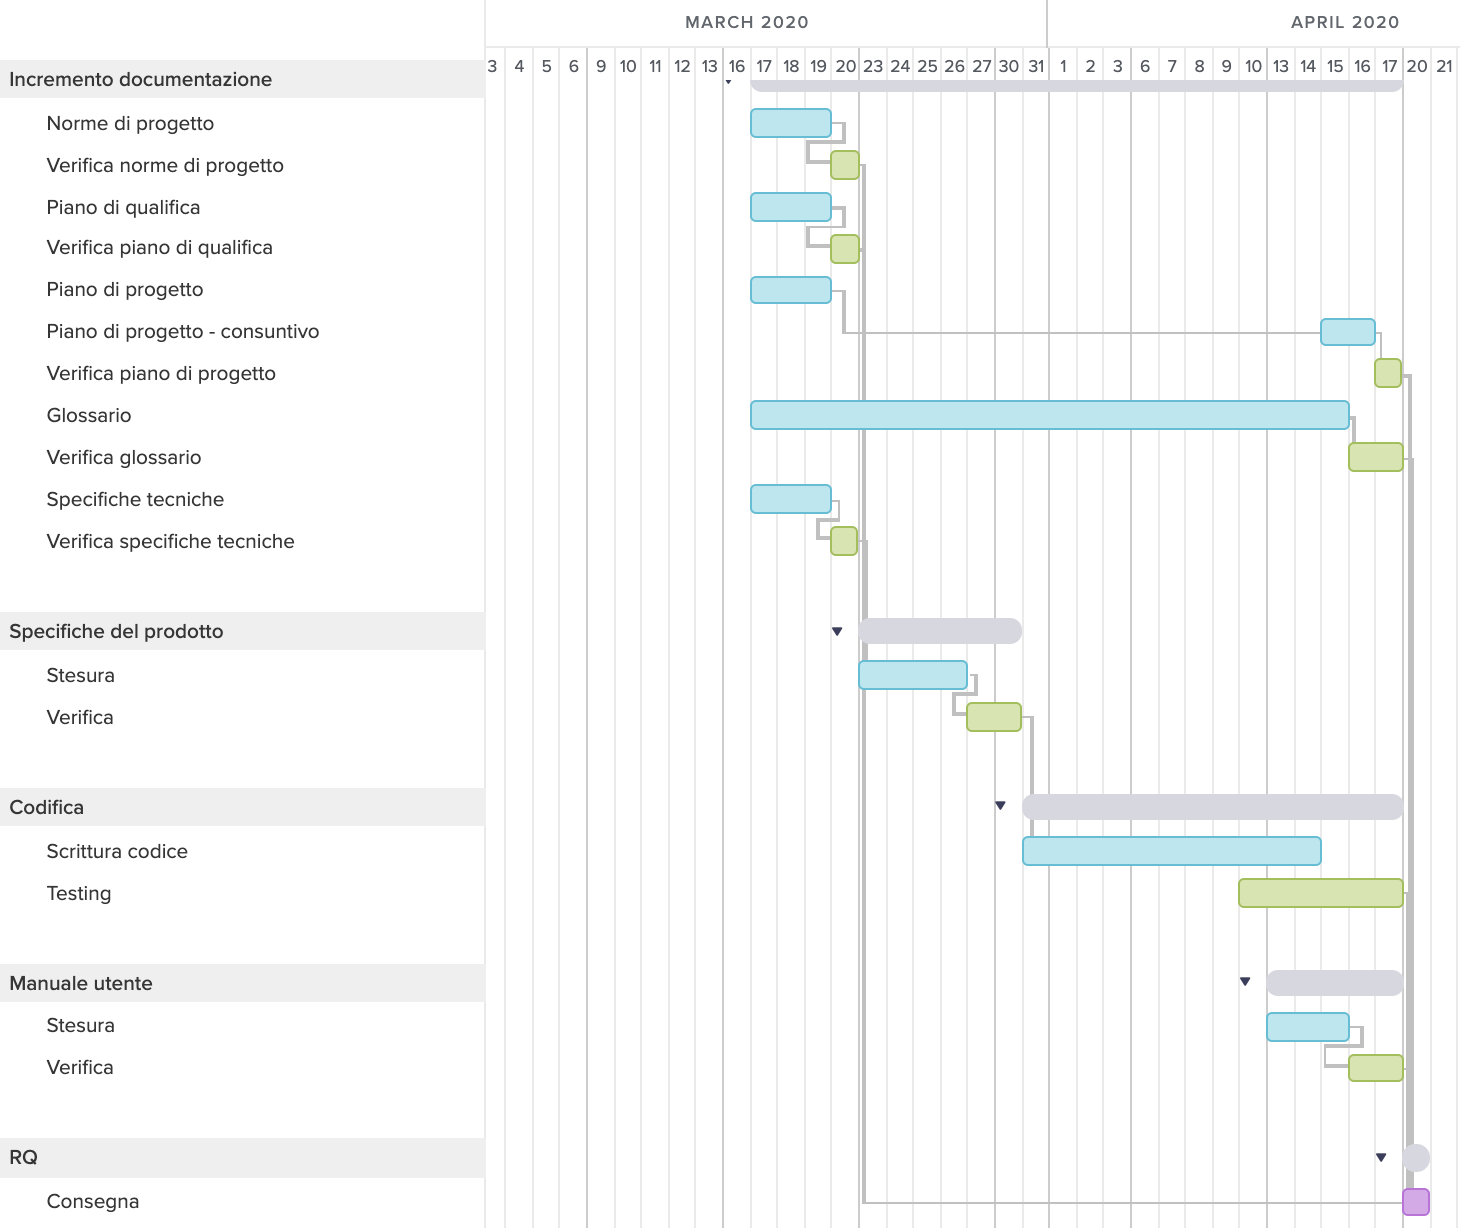
\includegraphics[width=\textwidth]{res/img/g4}
	\caption{Pianificazione Progettazione di dettaglio}
\end{figure}
\noindent Questa fase è stata suddivisa nelle attività:
\begin{itemize}
	\item \textbf{Specifiche di prodotto:} documento nel quale vengono individuate le unità che costituiscono il prodotto; viene eseguita una progettazione dettagliata in modo da permettere la successiva codifica delle funzionalità;
	\item  \textbf{Codifica:} implementazione del prodotto;
	\item \textbf{Manuale utente:} realizzazione del \textit{Manuale Utente} per l'utilizzo del prodotto;
	\item \textbf{Documentazione:} incremento della documentazione in base ai nuovi dati rilevati.
\end{itemize}

\subsection{Validazione e collaudo}
\begin{figure}[h!]
	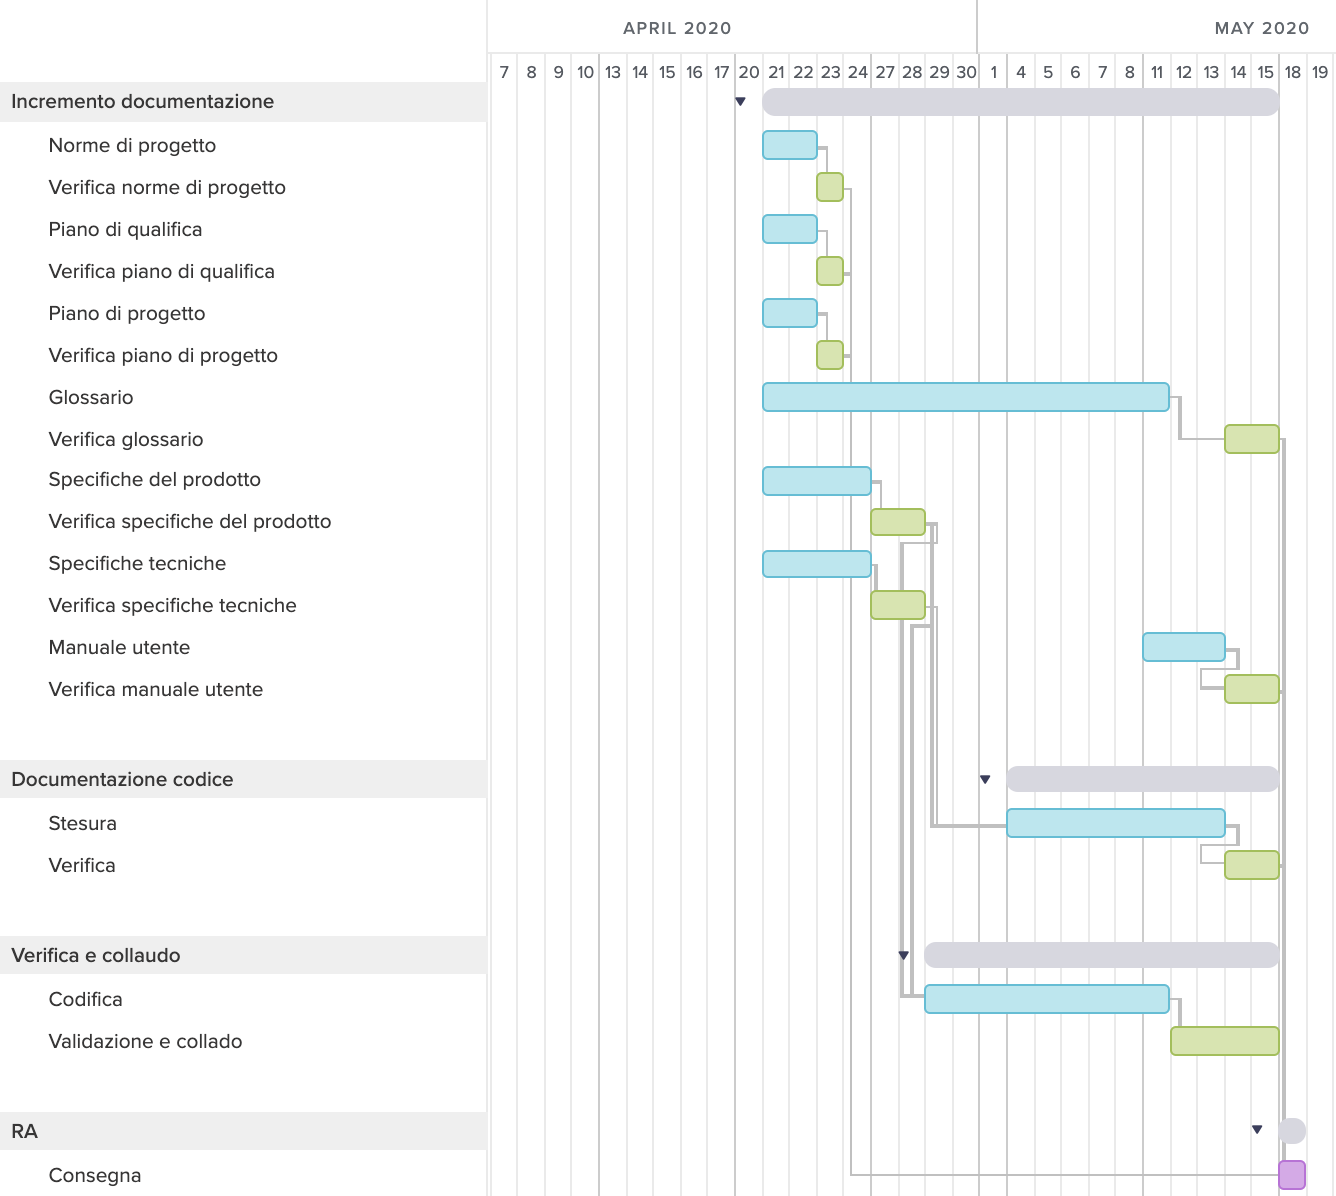
\includegraphics[width=\textwidth]{res/img/g5}
	\caption{Pianificazione Progettazione di dettaglio}
\end{figure}
Questa fase è stata suddivisa nelle attività:
\begin{itemize}
	\item \textbf{Documentazione codice:} realizzazione della documentazione relativa al codice scritto, con lo scopo di fornire informazioni necessarie alla manutenzione del software;
	\item \textbf{Validazione e Collaudo:} controlli per verificare la conformità alle del prodotto ai bisogni del cliente;
	\item \textbf{Documentazione:} incremento della documentazione in base ai nuovi dati rilevati.
\end{itemize}
